\documentclass[border=10pt]{standalone}

\usepackage[utf8]{inputenc}                                 % Codificação do documento
\usepackage[T1]{fontenc}                                    % Seleção de código de fonte
\usepackage{microtype}                                      % Melhora a justificação do documento
\usepackage{lmodern}                                        % Usa a fonte Latin Modern
\usepackage{ae, aecompl}                                    % Fontes de alta qualidade

\usepackage{amsmath}
\usepackage{verbatim}
\usepackage{tikz}
\usetikzlibrary{arrows,calc,positioning,shadows.blur,decorations.pathreplacing}
\usepackage{etoolbox}

\begin{document}
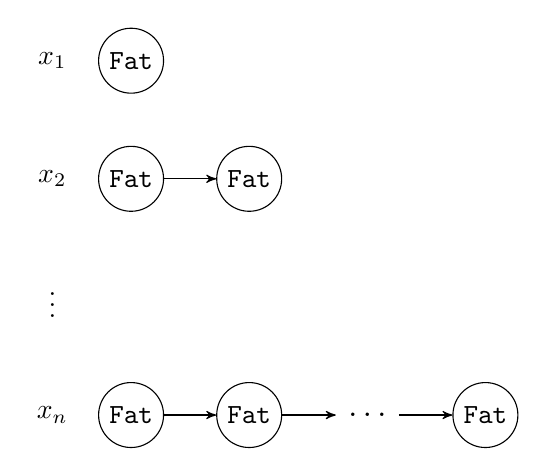
\begin{tikzpicture}
[
	              y = -1cm,
	           ->, >= stealth',
	  node distance = 2cm,
	  vertex/.style = { draw=black, circle, inner sep=2.5pt },
	   label/.style = { draw=none, fill=none },
	toplabel/.style = { label, anchor=south }
]
	% traces for fatorial
	\node (10) at (-1,0)   [label]    {$x_1$};
	\node (11) at  (0,0)   [vertex]   {\texttt{Fat}};

	\node (20) at  (-1,1.5)   [label]    {$x_2$};
	\node (21) at   (0,1.5)   [vertex]   {\texttt{Fat}};
	\node (22) at (1.5,1.5)   [vertex]   {\texttt{Fat}};
	\draw [->] (21) edge (22);

	\node (30) at  (-1,3)   [label]    {$\vdots$};

	\node (40) at  (-1,4.5)   [label]    {$x_n$};
	\node (41) at   (0,4.5)   [vertex]   {\texttt{Fat}};
	\node (42) at (1.5,4.5)   [vertex]   {\texttt{Fat}};
	\node (43) at   (3,4.5)   [label]    {\texttt{...}};
	\node (44) at (4.5,4.5)   [vertex]   {\texttt{Fat}};
	\draw [->] (41) edge (42) (42) edge (43) (43) edge (44);

\end{tikzpicture}
\end{document}